\documentclass{article}

% if you need to pass options to natbib, use, e.g.:
%     \PassOptionsToPackage{numbers, compress}{natbib}
% before loading neurips_2024


% ready for submission
% \usepackage{neurips_2024}


% to compile a preprint version, e.g., for submission to arXiv, add add the
% [preprint] option:
     \usepackage[preprint]{neurips_2024}


% to compile a camera-ready version, add the [final] option, e.g.:
%     \usepackage[final]{neurips_2024}


% to avoid loading the natbib package, add option nonatbib:
%    \usepackage[nonatbib]{neurips_2024}


\usepackage[utf8]{inputenc} % allow utf-8 input
\usepackage[T1]{fontenc}    % use 8-bit T1 fonts
\usepackage{hyperref}       % hyperlinks
\usepackage{url}            % simple URL typesetting
\usepackage{booktabs}       % professional-quality tables
\usepackage{amsfonts}       % blackboard math symbols
\usepackage{nicefrac}       % compact symbols for 1/2, etc.
\usepackage{microtype}      % microtypography
\usepackage{xcolor}         % colors
\usepackage{amsmath}
\usepackage{natbib}
\usepackage{graphicx}  % For including graphics
\usepackage{float}     % To control figure placement



\title{Deep Learning 1 - Homework 1}


% The \author macro works with any number of authors. There are two commands
% used to separate the names and addresses of multiple authors: \And and \AND.
%
% Using \And between authors leaves it to LaTeX to determine where to break the
% lines. Using \AND forces a line break at that point. So, if LaTeX puts 3 of 4
% authors names on the first line, and the last on the second line, try using
% \AND instead of \And before the third author name.


\author{%
  Pedro M.P.~Curvo \\
  MSc Artificial Intelligence\\
  University of Amsterdam\\
  \texttt{pedro.pombeiro.curvo@student.uva.nl} \\
  % examples of more authors
  % \And
  % Coauthor \\
  % Affiliation \\
  % Address \\
  % \texttt{email} \\
  % \AND
  % Coauthor \\
  % Affiliation \\
  % Address \\
  % \texttt{email} \\
  % \And
  % Coauthor \\
  % Affiliation \\
  % Address \\
  % \texttt{email} \\
  % \And
  % Coauthor \\
  % Affiliation \\
  % Address \\
  % \texttt{email} \\
}


\begin{document}


\maketitle


% \begin{abstract}
%   The abstract paragraph should be indented \nicefrac{1}{2}~inch (3~picas) on
%   both the left- and right-hand margins. Use 10~point type, with a vertical
%   spacing (leading) of 11~points.  The word \textbf{Abstract} must be centered,
%   bold, and in point size 12. Two line spaces precede the abstract. The abstract
%   must be limited to one paragraph.
% \end{abstract}


\section*{Question 1}

\subsection*{a) b) c)}

The linear model described previously can be written as:

\begin{equation}
    Y = X W^T + B
\end{equation}

Where $Y$ is the output, $X$ is the input, $W$ is the weight matrix and $B$ is the bias, with
$Y \in \mathbb{R}^{S \times N}$, $X \in \mathbb{R}^{S \times M}$, $W \in \mathbb{R}^{N \times M}$ and $B \in \mathbb{R}^{S \times N}$.

In order to compute $\frac{\partial L}{\partial W}$, we can use the chain rule:

\begin{align*}
    \left[ \frac{\partial L}{\partial W} \right]_{ij} &= \sum_{k, l} \frac{\partial L}{\partial Y_{kl}} \frac{\partial Y_{kl}}{\partial W_{ij}} \quad \text{, by the partial derivative chain rule} \\
    &= \sum_{k, l} \frac{\partial L}{\partial Y_{kl}} \frac{\partial}{\partial W_{ij}} \left( \sum_{m=1}^{M} X_{km} W_{ml} + B_{kl} \right) \\
    &= \sum_{k, l} \frac{\partial L}{\partial Y_{kl}} \cdot X_{ki} \delta_{lj} \\
    &= \sum_{k} \frac{\partial L}{\partial Y_{kj}} X_{ki} \\
\end{align*}

Which can be written as:


\begin{equation}
    \frac{\partial L}{\partial W} = \frac{\partial L}{\partial Y}^T X
\end{equation}

% \begin{align*}
%     \frac{\partial L}{\partial W} &= \frac{\partial L}{\partial Y}^T \frac{\partial Y}{\partial W} \quad \text{, an explanation for the transpose is given below} \\
%     &= \frac{\partial L}{\partial Y}^T \frac{\partial (XW^T + B)}{\partial W} \quad \text{(from equation 1)} \\
%     &= \frac{\partial L}{\partial Y}^T \frac{\partial (XW^T)}{\partial W} \quad \text{(since B does not depend on W)} \\
%     &= \frac{\partial L}{\partial Y}^T X
% \end{align*}

% Here, we used the transpose of $\frac{\partial L}{\partial Y}$ since we are dealing with batches of data. Indeed,
% if we confirm, $\frac{\partial L}{\partial Y}$ would have the same dimensions as $Y$, which is $\mathbb{R}^{S \times N}$.
% And $X$ has dimensions $\mathbb{R}^{S \times M}$. Hence, to compute the matrix product, we need to transpose $\frac{\partial L}{\partial Y}$.
% We don't transpose $X$ because then we would end up with a gradient that does not match the required dimensions for $W$.
% Also, it makes sense for the batches to be the inner dimensions of the matrix product, since we want to have a sum over the samples.

Similarly, to compute $\frac{\partial L}{\partial B}$, we can use the chain rule:

\begin{align*}
    \left[ \frac{\partial L}{\partial B} \right]_{ij} &= \sum_{k, l} \frac{\partial L}{\partial Y_{kl}} \frac{\partial Y_{kl}}{\partial B_{ij}} \\
    &= \sum_{k, l} \frac{\partial L}{\partial Y_{kl}} \frac{\partial}{\partial B_{ij}} \left( \sum_{m=1}^{M} X_{km} W_{ml} + B_{kl} \right) \\
    &= \sum_{k, l} \frac{\partial L}{\partial Y_{kl}} \cdot \delta_{ki} \delta_{lj} \\
    &= \sum_{k} \frac{\partial L}{\partial Y_{kj}} \delta_{ki} \\ 
    &= \frac{\partial L}{\partial Y_{ij}}
\end{align*}

Which can be written as:

\begin{equation}
    \frac{\partial L}{\partial B} = \frac{\partial L}{\partial Y}
\end{equation}

Now, it is noted in the question that $B_{ij} = b_j$ for all $i$. Hence:

\begin{align*}
    \frac{\partial L}{\partial b_j} = \frac{\partial L}{\partial B_{ij}} = \frac{\partial L}{\partial Y_{ij}} \quad \forall i
\end{align*}

This because the bias $B$ has a row-vector structure, with the same bias for all samples in the batch. And, indeed,
we get a row vector as the gradient of the bias if we choose any row $i$ of the gradient of $B$, which is the same as
a row of the gradient of $Y$.

% \begin{align*}
%     \frac{\partial L}{\partial B} &= \frac{\partial L}{\partial Y} \frac{\partial Y}{\partial B} \\
%     &= \frac{\partial L}{\partial Y} \frac{\partial (XW^T + B)}{\partial B} \quad \text{(from equation 1)} \\
%     &= \frac{\partial L}{\partial Y} \frac{\partial B}{\partial B} \quad \text{(since B does not depend on W)} \\
%     &= \sum_{i=1}^{S} \frac{\partial L}{\partial Y_i}
% \end{align*}

Finally, to compute $\frac{\partial L}{\partial X}$:

\begin{align*}
    \left[ \frac{\partial L}{\partial X} \right]_{ij} &= \sum_{k, l} \frac{\partial L}{\partial Y_{kl}} \frac{\partial Y_{kl}}{\partial X_{ij}} \\
    &= \sum_{k, l} \frac{\partial L}{\partial Y_{kl}} \frac{\partial}{\partial X_{ij}} \left( \sum_{m=1}^{M} X_{km} W_{ml} + B_{kl} \right) \\
    &= \sum_{k, l} \frac{\partial L}{\partial Y_{kl}} \cdot W_{lj} \delta_{ki} \\
    &= \sum_{l} \frac{\partial L}{\partial Y_{il}} W_{lj}
\end{align*}


Which can be written as:

\begin{equation}
    \frac{\partial L}{\partial X} = \frac{\partial L}{\partial Y} W
\end{equation}

\textbf{Note:} We swapped the dimensions of $W$ because, without the summation, the formula is given
by the matrix product $W^T$. Hence, the first index of $W$, which was supposed to be $j$ goes to $M$. However, this is
actually the second dimension of $W$, hence we need to swap the dimensions of $W$. This can be checked by the dimensions
of the resulting gradient.

% \begin{align*}
%     \frac{\partial L}{\partial X} &= \frac{\partial L}{\partial Y} \frac{\partial Y}{\partial X} \\
%     &= \frac{\partial L}{\partial Y} \frac{\partial (XW^T + B)}{\partial X} \quad \text{(from equation 1)} \\
%     &= \frac{\partial L}{\partial Y} \frac{\partial (XW^T)}{\partial X} \quad \text{(since W and X does not depend on B)} \\
%     &= \frac{\partial L}{\partial Y} W
% \end{align*}

\newpage
\subsection*{d)}

Considering the element-wise activation h, given by: 

\begin{align*}
    Y = h(X) \Rightarrow  Y_{ij} = h(X_{ij})
\end{align*}

By applying the chain rule, we can compute $\frac{\partial L}{\partial X}$ as follows:

\begin{align*}
    \frac{\partial L}{\partial X_{ij}} &= \sum_{k, l}\frac{\partial L}{\partial Y_{kl}} \frac{\partial Y_{kl}}{\partial X_{ij}} \\
    &= \sum_{k, l}\frac{\partial L}{\partial Y_{kl}} \frac{\partial h(X_{kl})}{\partial X_{ij}} \\
    &= \sum_{k, l}\frac{\partial L}{\partial Y_{kl}} \frac{\partial h(X_{kl})}{\partial X_{kl}} \delta_{ki} \delta_{lj} \quad \text{, since $h$ is element-wise} \\
    &= \frac{\partial L}{\partial Y_{ij}} \frac{\partial h(X_{ij})}{\partial X_{ij}}
\end{align*}

Which can have a simple notation of:

\begin{align*}
    \frac{\partial L}{\partial X_{ij}} = \frac{\partial L}{\partial Y_{ij}} \cdot h'(X_{ij})
\end{align*}

where $h'(X)$ is the derivative of the activation function h with respect to their input. 

Now, this rule is applied to all elements of the matrix X, resulting in the following:

\begin{align*}
    \frac{\partial L}{\partial X} = \frac{\partial L}{\partial Y} \odot h'(X)
\end{align*}

where $\odot$ is the Hadamard product and $h'$ is applied element-wise to the matrix X.

As we can see, since we are applying the Hadamard product on a derivative that is also applied element-wise,
the result will have the same dimensions as the input matrix X. Hence, $\frac{\partial L}{\partial X} \in \mathbb{R}^{S \times M}$.

\newpage
\subsection*{e)}

As presented, the gradients can be given by: 

\begin{align*}
    \frac{\partial L}{\partial Z} = Y \odot \left( \frac{\partial L}{\partial Y} - \left( \frac{\partial L}{\partial Y} \odot Y \right) 1 1^T \right) \\
    \frac{\partial L}{\partial Y} = - \frac{1}{S} \left( \frac{T}{Y} \right)
\end{align*}

First, we began by replacing the expression for $\frac{\partial L}{\partial Y}$ in the expression for $\frac{\partial L}{\partial Z}$:

\begin{align*}
    \frac{\partial L}{\partial Z} = Y \odot \left( - \frac{1}{S} \left( \frac{T}{Y} \right) - \left( - \frac{1}{S} \left( \frac{T}{Y} \right) \odot Y \right) 1 1^T \right)
\end{align*}

Now, since $- \frac{1}{S}$ is a scalar, we can take it out of the Hadamard product:

\begin{align*}
    \frac{\partial L}{\partial Z} = - \frac{1}{S} Y \odot \left( \frac{T}{Y} - \left( \frac{T}{Y} \odot Y \right) 1 1^T \right)
\end{align*}

Now, we can use the distributive property of the Hadamard product to simplify the expression:

\begin{align*}
    \frac{\partial L}{\partial Z} = - \frac{1}{S} \left( Y \odot \frac{T}{Y} - Y \odot \left( \left( \frac{T}{Y} \odot Y \right) 1 1^T \right) \right)
\end{align*}

Now, since the division is element-wise, we can cancel out the Hadamard product with the element-wise division:

\begin{align*}
    \frac{\partial L}{\partial Z} = - \frac{1}{S} \left( T - Y \odot \left( \left( T \right) 1 1^T \right) \right)
\end{align*}

Now, we need to look at the matrix product of $T 1 1^T$. $1 1^T$ gives us a matrix of ones, with dimensions $C \times C$.
Naming the result as $H$, we have that: 

\begin{align*}
    H_{ij} = \sum_{k=1}^{C} T_{ik} 1 = \sum_{k=1}^{C} T_{ik}
\end{align*}

But since $T$ is a one-hot encoded matrix, we have that $\sum_{j} T_{ij} = 1$. Hence, $H_{ij} = 1$ for all $i$ and $j$.

Now, we can simplify the expression for $\frac{\partial L}{\partial Z}$:

\begin{align*}
    \frac{\partial L}{\partial Z} &= - \frac{1}{S} \left( T - Y \odot H \right) \\
    &= - \frac{1}{S} \left( T - Y \right) \\
    &= \frac{1}{S} \left( Y - T \right)
\end{align*}

With that, we can infer that: 

\begin{align*}
    \alpha = \frac{1}{S} \\
    M = Y - T
\end{align*}

Since S is the number of samples, then $\alpha \in \mathbb{R}^{+}$ as we wanted to show.

\section*{Question 2}

% Insert two images, one is the train loss and the other the validation accuracy, side by side

\begin{figure}[H]
    \centering
    \begin{minipage}{0.45\textwidth}
        \centering
        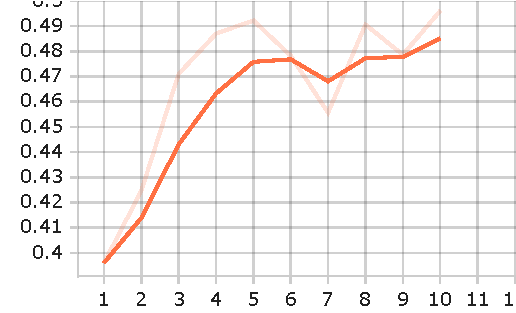
\includegraphics[width=\linewidth]{images/numpy/Accuracy_val.pdf}
        \caption{Validation Accuracy}
    \end{minipage} \hfill
    \begin{minipage}{0.45\textwidth}
        \centering
        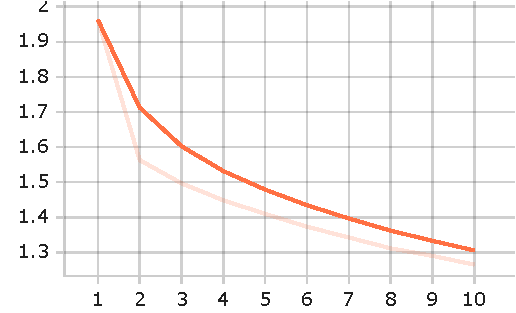
\includegraphics[width=\linewidth]{images/numpy/Loss_train.pdf}
        \caption{Train Loss}
    \end{minipage}
    \caption{Test Accuracy: 49.72\%}
\end{figure}



\section*{Question 3}

\begin{figure}[H]
    \centering
    \begin{minipage}{0.45\textwidth}
        \centering
        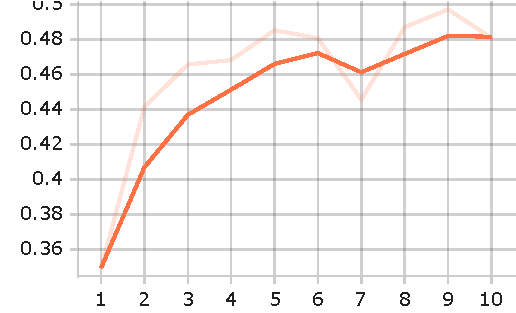
\includegraphics[width=\linewidth]{images/torch_nonorm/Accuracy_validation.pdf}
        \caption{Validation Accuracy}
    \end{minipage} \hfill
    \begin{minipage}{0.45\textwidth}
        \centering
        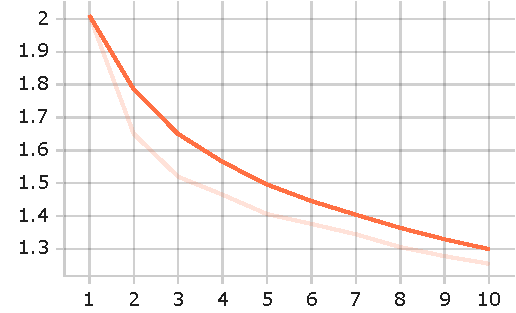
\includegraphics[width=\linewidth]{images/torch_nonorm/Loss_train-2.pdf}
        \caption{Train Loss}
    \end{minipage}
    \caption{Test Accuracy: 48.60\%}
\end{figure}

\newpage
\section*{Question 4}

\subsection*{a)}

To show that the eigenvalues for the Hessian matrix in a strictly local minimum are all positive, 
we need to began by showing that the Hessian matrix is positive-definite at that point.

Let $f: \mathbb{R}^n \rightarrow \mathbb{R}$ be a function that is twice differentiable in an open neighborhood at a point $x^*$, hence
$f \in C^2$. Assuming that $x^*$ is a local minimum, we have that $\nabla f(x^*) = 0$, since if $x^*$ is a local extremum,
the gradient must be zero.

If we know expand the Taylor series of $f$ around $x^*$, we have that:

\begin{align*}
    f(x + \lambda d) &= f(x) + \lambda \nabla f(x)^T d + \frac{1}{2} \lambda^2 d^T H_f(x) d + o(\lambda^2 d^T d) \\
    &= f(x) + \frac{1}{2} \lambda^2 d^T H_f(x) d + o(\lambda^2 d^T d)
\end{align*}

Because $x^*$ is a strictly local minimum, we have that, by definition:

\begin{align*}
    0 &< \lim_{\lambda \rightarrow 0} \frac{f(x^* + \lambda d) - f(x^*)}{\lambda^2} \quad \text{because for a strictly local minimum, $f(x) > f(x^*)$ for all $x$ in the neighborhood of $x^*$} \\
    &= \lim_{\lambda \rightarrow 0} \frac{f(x^*) + \frac{1}{2} \lambda^2 d^T H_f(x^*) d + o(\lambda^2 d^T d) - f(x^*)}{\lambda^2} \\
    &= \frac{1}{2} d^T H_f(x^*) d
\end{align*}

This is true for all $d \neq 0$.

Now, by the definition of positive-definite matrix:

\begin{align*}
    d^T H_f(x^*) d > 0 \quad \text{for all $d \neq 0$}
\end{align*}

Hence, if the Hessian matrix is positive-definite at a point $x^*$, then $x^*$ is a strictly local minimum,
by the definitions above. Notice, however, that is not true the other way around, since a strictly local minimum
can have a positive semi-definite Hessian matrix. Having a positive definite Hessian matrix is a sufficient condition
for a strictly local minimum, but not a necessary condition. I'm going to assume from now on that the question
was asking that if we have a Hessian positive definite in a point $x^*$, then $x^*$ is a strictly local minimum.

Now, to proof the statement, we need to show that all the eigenvalues of a positive-definite matrix are positive.

If we start by assuming that there is one eigenvalue $\lambda$ that is negative, then for its corresponding eigenvector $v$:

\begin{align*}
    v^T H v &= \lambda v^T v \\
    &= \lambda ||v||^2 < 0 \quad \text{(since $\lambda < 0$) and $||v||^2 > 0$)}
\end{align*}

This contradicts the definition of positive-definite matrix.

Now, if we assume that there is one eigenvalue $\lambda$ that is zero, then for its corresponding eigenvector $v$:

\begin{align*}
    v^T H v &= \lambda v^T v \\
    &= 0 \quad \text{(since $\lambda = 0$)}
\end{align*}

Which also contradicts the definition of positive-definite matrix.

Hence, all the eigenvalues of a positive-definite matrix are positive. We can than conclude, that
if we have a Hessian matrix that is positive-definite at a point $x^*$, then $x^*$ is a strictly local minimum.
To proof the necessary condition, then H is positive-semidefinite at $x^*$ and we only need to do the first step of the proof
above. 

\subsection*{b)}

Let $f: \mathbb{R}^n \rightarrow \mathbb{R}$ be a function that is twice differentiable at a point $p$. If $p$
is a strictly local minimum, we have that $H_f(p)$ is positive-definite with all $n$ eigenvalues positive.

Now, if we think that the eigenvalues can assume two possible states, we have that the number of possible states is $2^n$.
With this, only one configuration is possible, which is the one where all the eigenvalues are positive, hence
the probability of this configuration is $\frac{1}{2^n}$.

Now, for the saddle points, we have that the Hessian matrix is indefinite, with both positive and negative eigenvalues, Hence,
we have $2^n - 2$ possible configurations (all the states minus the one with all positive eigenvalues and the one with all negative eigenvalues). With
probability $\frac{2^n - 2}{2^n}$. 

This shows that the number of saddle points is exponentially larger than the number of local minima as
we wanted to show.

\subsection*{c)}

A saddle points $p$ has the property of having its gradient equal to zero, $\nabla f(p) = 0$.
Now, by taking the formula of gradient descent, we have that:

\begin{align*}
    p^{\tau+1} = p^{\tau} - \eta  \nabla f(p^\tau)
\end{align*}

Since, $\nabla f(p) = 0$, we have that $p^{\tau+1} = p^{\tau}$. Hence, the algorithm will not move from the saddle point.
This is a problem, since the algorithm will be stuck at the saddle point and will not be able to converge to a minima.
Besides that, for points close to the saddle point, the gradient will be small, making it hard for the algorithm to escape
that locality, since $p^{\tau+1} \approx p^{\tau}$.


\newpage
\section*{Question 5}

\subsection*{a)}

Taking the derivative of $L$ with respect to $\gamma_i$:

\begin{align*}
    \frac{\partial L}{\partial \gamma_i} &= \frac{\partial L}{\partial y_i} \frac{\partial y_i}{\partial \gamma_i} \\
    &= \frac{\partial L}{\partial y_i} \frac{\partial}{\partial \gamma_i} \left( \gamma_i x_i + \beta_i \right) \\
    &= \frac{\partial L}{\partial y_i} x_i
\end{align*}

Since the batch norm is applied in a batch, we have that: 

\begin{align*}
    \frac{\partial L}{\partial \gamma_i} = \sum_{j=1}^{S} \frac{\partial L}{\partial y_i^{(j)}} x_i^{(j)}
\end{align*}

Where $S$ is the number of samples in the batch and $y_i^{(j)}$ is the output of the $i$-th neuron for the $j$-th sample
and $x_i^{(j)}$ is the input of the $i$-th neuron for the $j$-th sample.

Taking the derivative of $L$ with respect to $\beta_i$:

\begin{align*}
    \frac{\partial L}{\partial \beta_i} &= \frac{\partial L}{\partial y_i} \frac{\partial y_i}{\partial \beta_i} \\
    &= \frac{\partial L}{\partial y_i} \frac{\partial}{\partial \beta_i} \left( \gamma_i x_i + \beta_i \right) \\
    &= \frac{\partial L}{\partial y_i} \cdot 1 \\
\end{align*}

Since the batch norm is applied in a batch, we have that:

\begin{align*}
    \frac{\partial L}{\partial \beta_i} = \sum_{j=1}^{S} \frac{\partial L}{\partial y_i^{(j)}}
\end{align*}

\newpage
\subsection*{b)}

Since we have a linear connected layer with input since 20 and output size 40, we have that $x \in \mathbb{R}^{20}$ and $y \in \mathbb{R}^{40}$.
Hence, the weight matrix $W$ has dimensions $40 \times 20$ and the bias $B$ has dimensions $1 \times 40$.
This makes the number of parameters in the linear layer $40 \times 20 + 40 = 840$.

Now, for the batch norm, we have that $\gamma \in \mathbb{R}^{40}$ and $\beta \in \mathbb{R}^{40}$, 
since they have the same dimensions as the output of the linear layer. Hence, the number of parameters in the batch norm layer is $40 + 40 = 80$.

This makes the total number of parameters in the network $840 + 80 = 920$.

\newpage
\subsection*{c)}

Batch Normalization, as the name indicates, normalizes the activations of the neurons in a batch to have
zero mean and unit variance during training, which helps stabilize the training process. However, during training
we usually are passing batches of data through the network with the same dimensions, but during inference we might
be passing single samples through the network or smaller batches. This poses a problem, since the the variance and
mean of a smaller batch might not be representative of the ones during training. Besides that, for small batch sizes
or single samples, normalization fails due to the lack of statistics. To solve this problem, Batch Normalization
layers usually have two modes, one for training and one for inference. During training, the layer computes the mean
and variance of the batch and normalizes the activations and keeps a running average of the mean and variance. During
inference, the layer uses the running average of the mean and variance from the training to normalize the activations.
This solution is presented in PyTorch as indicated by~\citep{BatchNorm1d} and originally proposed by~\citep{Ioffe_Szegedy_2015}.

\subsection*{d)}

A dead neuron has the property that outputs zero for all inputs after a certain time during training
becoming inactive and statics, since the weights are not updated anymore. This neuron then does not contribute
to the learning process and can be seen as a waste of resources. This dead neurons are common in ReLU activation. 
This can be explained by the fact that the ReLU activation function is defined as $h(x) = max(0, x)$, which means that
during training, if the input of the neuron is negative, which can be caused by negative weights or
negative updates on the weights, the neuron will output zero and the weights will not be updated anymore because
the gradient will be zero, by the chain rule. This means that this neuron does not contribute either to the output
or either to the update of the weights.
Dead neurons are harmful to the training process, since they become a waste of computational resources and decrease
the capacity of the network, by reducing the number of neurons that are actually learning and by reducing the capacity
of updating the weights. It can also lead that during training, the network will dispose features in layers
that might be important for the learning process.

\subsection*{e)}

As presented in the previous question, in the case of ReLU activation, dead neurons can be caused by negative inputs to
the layer. Well, if we have all negative inputs to the layer, the output of the layer will be zero, leading
to the dead neuron problem. However, by using a Batch Normalization layer, we can avoid this problem. This is because
the Batch Normalization layer normalizes the activations of the neurons to have zero mean and unit variance, meaning
that, even with all negative inputs, the Batch Normalization layer will guarantee that half of the neurons will have
positive outputs. With this, we prevent a zero output on the neuron and avoid the dead neuron problem.

\newpage
\subsection*{f)}

\begin{figure}[H]
    \centering
    \begin{minipage}{0.45\textwidth}
        \centering
        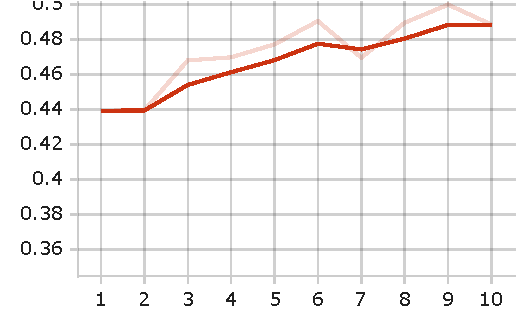
\includegraphics[width=\linewidth]{images/torch_norm/Accuracy_validation-2.pdf}
        \caption{Validation Accuracy}
    \end{minipage} \hfill
    \begin{minipage}{0.45\textwidth}
        \centering
        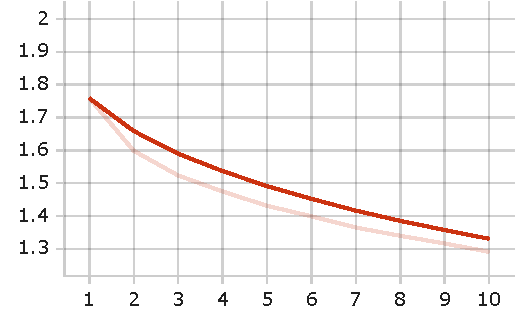
\includegraphics[width=\linewidth]{images/torch_norm/Loss_train-3.pdf}
        \caption{Train Loss}
    \end{minipage}
    \caption{Test Accuracy: 49.65\%}
\end{figure}

As we can see, the Batch Normalization layer improved the performance of the network, with a test accuracy of 49.65\%
compared to the 48.60\% of the network without the Batch Normalization layer. We also observe that the network with
the Batch Normalization layer converged faster than the network without the Batch Normalization layer, since
it reached the same accuracy in fewer epochs.

This can be explained by the fact that the Batch Normalization layer
might have prevented some dead neurons, making the network more efficient and faster to train with more neurons
contributing to the learning process and also because the Batch Normalization layer functions
as a regularization technique, by preventing two high weights and activations. This can be seen in the graphs
of the train loss and validation accuracy, where the network with the Batch Normalization layer has a smoother
curve. 
The Batch Normalization layer also helps keeping an internal covariance shift, preventing diverging gradients.





\bibliographystyle{abbrvnat}
\bibliography{references} 


\end{document}